\documentclass[12pt,oneside,a4]{article}
\usepackage{float}
\usepackage[utf8]{inputenc}
\usepackage[a4paper,width=160mm,top=25mm,bottom=25mm]{geometry}
% \usepackage[lining,tabular]{fbb} % so math uses tabular lining figures
\usepackage{graphicx}
\usepackage{enumitem}
\usepackage{pdflscape}
\usepackage[table]{xcolor}
\usepackage{booktabs}
\usepackage{chngpage}
\usepackage{scrextend}

\usepackage{geometry}
\usepackage{tikz}
\usepackage{array}


\usepackage[hidelinks]{hyperref}
\graphicspath{{figures/}} %Setting the graphicspath
\renewcommand\abstractname{\large Introduction}

\renewcommand{\familydefault}{\sfdefault}
\let\tempone\itemize
\let\temptwo\enditemize
\renewenvironment{itemize}{\tempone\addtolength{\itemsep}{-0.5\baselineskip}}{\temptwo}

\newcommand{\linkdeploy}{https://pie2021-flightassistant-v19.herokuapp.com/}


\title{PIE Flight Assistant -- Quick Start Guide\\ \vspace{.2em} \large{ISAE-SUPAERO} \\ \small{v. 2022-02}\\ \vspace{-4em}}
\author{
    }
\date{}

\begin{document}

\maketitle
\vfill
\begin{center}
    \fbox{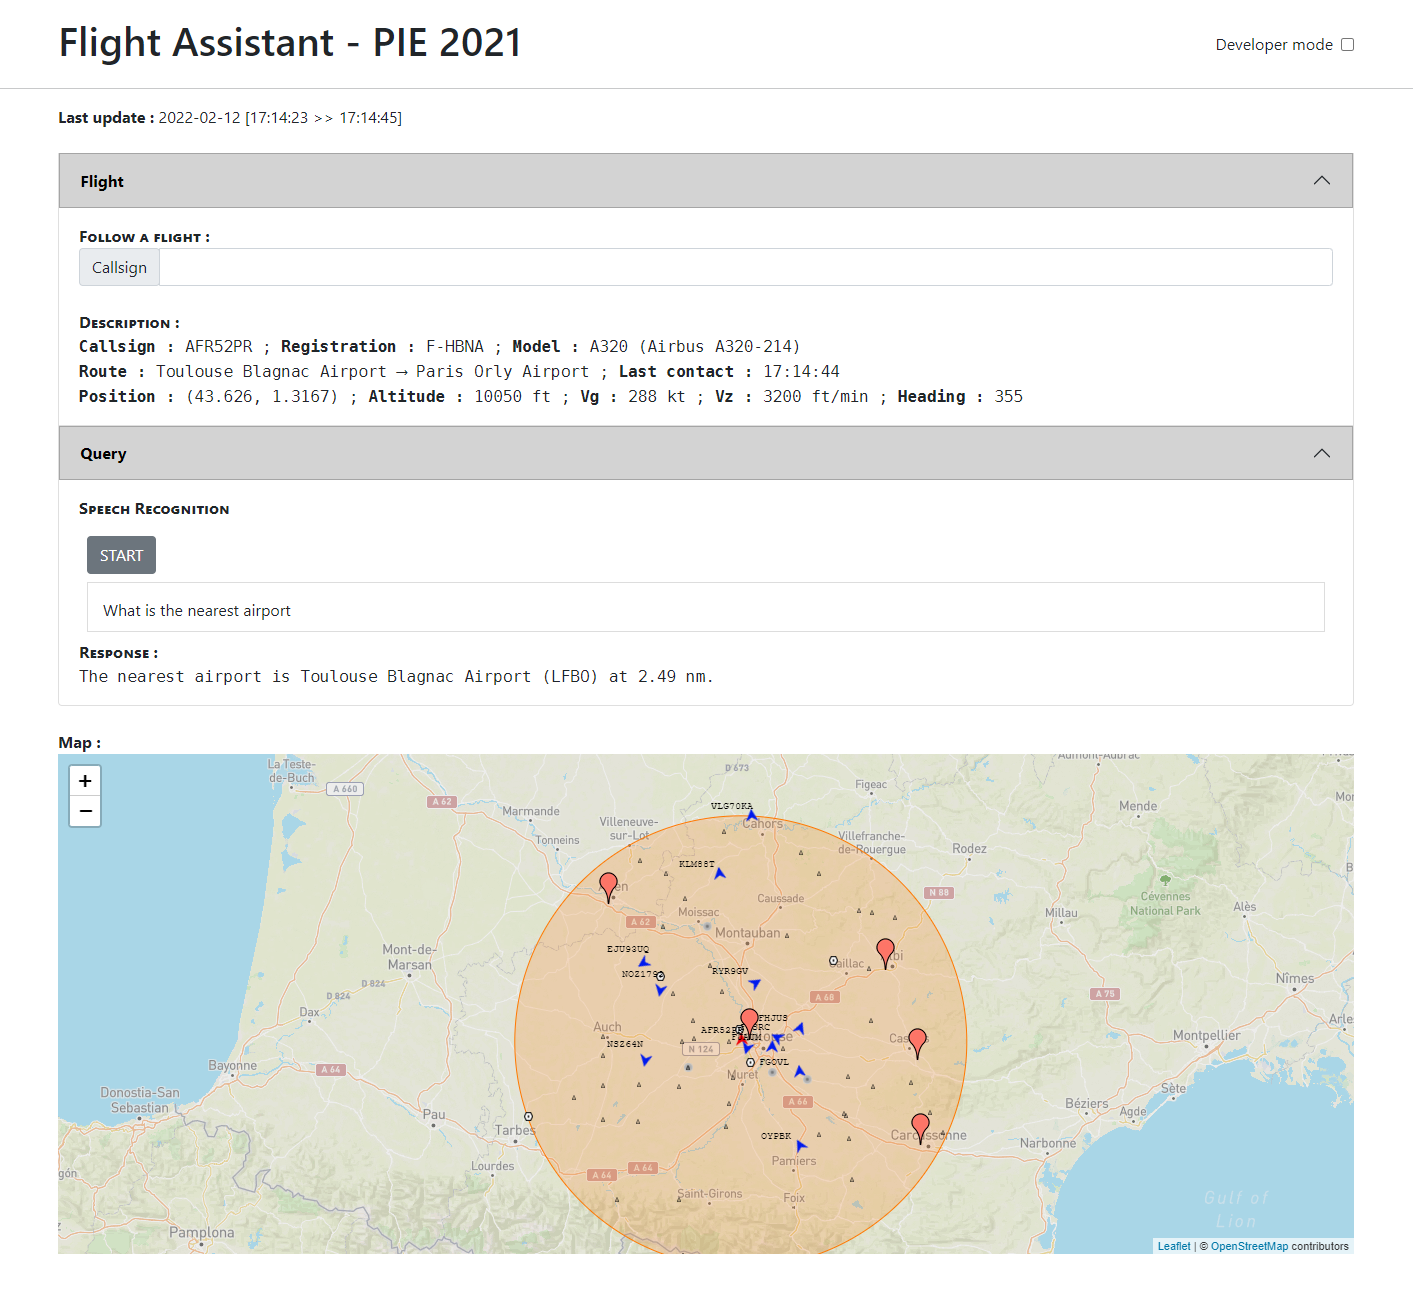
\includegraphics[width=.9\linewidth]{app.png}}
\end{center}
\vfill

\begin{abstract}
This project is an implementation of a flight assistant prototype towards mono-pilot cockpits.
The flight assistant aims at answering requests, eventually said in natural language by the pilot,
about its current status, or about information on diverse locations.
Data provided in this app are real-time data.

In the context of this prototype, you will be asked to select a flight and ask requests
as if you were the pilot of this flight.
The app is available here:
\begin{center}
    \vspace{-.5em}
    \url{\linkdeploy}
    \vspace{-.5em}
\end{center}
\end{abstract}

\clearpage
\tableofcontents

\clearpage

% ------------------------------------------------------------------------------

\section{Quick start}

\subsection{Required tools}
\begin{itemize}
    \item \textbf{Chrome} web browser is needed
    \item Microphone
\end{itemize}

\subsection{App launch}
\begin{itemize}
    \item Go to the following webpage : 
    \begin{center}
        \vspace{-.4em}
        \url{\linkdeploy}
    \end{center}
    \textit{You might wait for about 1 minute when you launch the app for the first time}
    \item Allow access to the microphone
\end{itemize}

\subsection{Flight following}

\begin{itemize}
    \item Select a flight to follow it. The easiest way is to click on one of the blue cursors representing the flights on the map (Figure~\ref{fig:select_flight}). 
    Else, you can search a flight by its callsign in the ``Follow a flight'' field (Figure~\ref{fig:search_flight})
    \begin{figure}[h!]
        \centering
        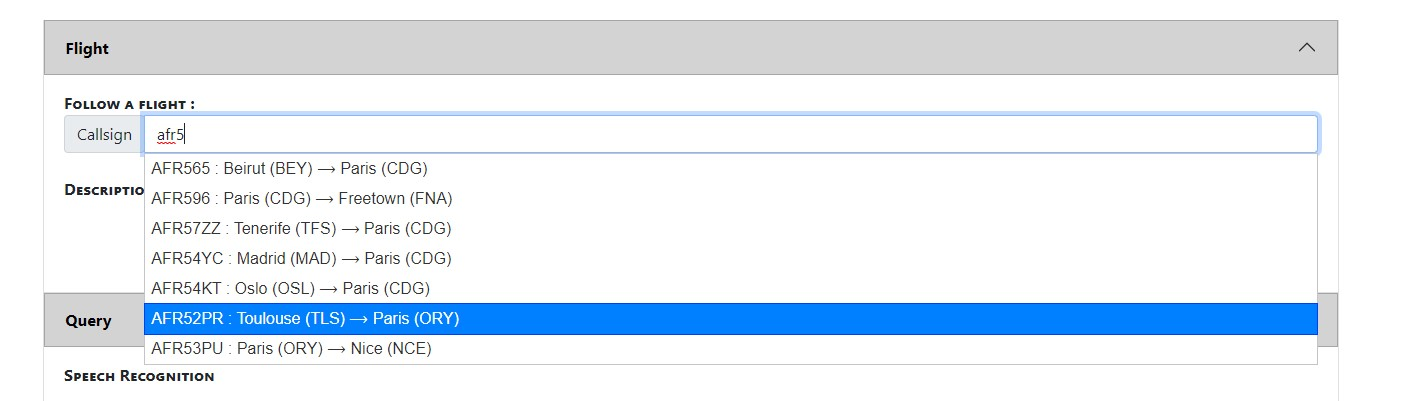
\includegraphics[width=.98\linewidth]{search_flight.jpg}
        \caption{Flight search by callsign}
        \label{fig:search_flight}
    \end{figure}
    \item On the map you may see that the orange zone in the map is centered on the selected flight
    \item The ``START'' button in the Speech Recognition section is also activated.
\end{itemize}

\begin{figure}[h!]
    \centering
    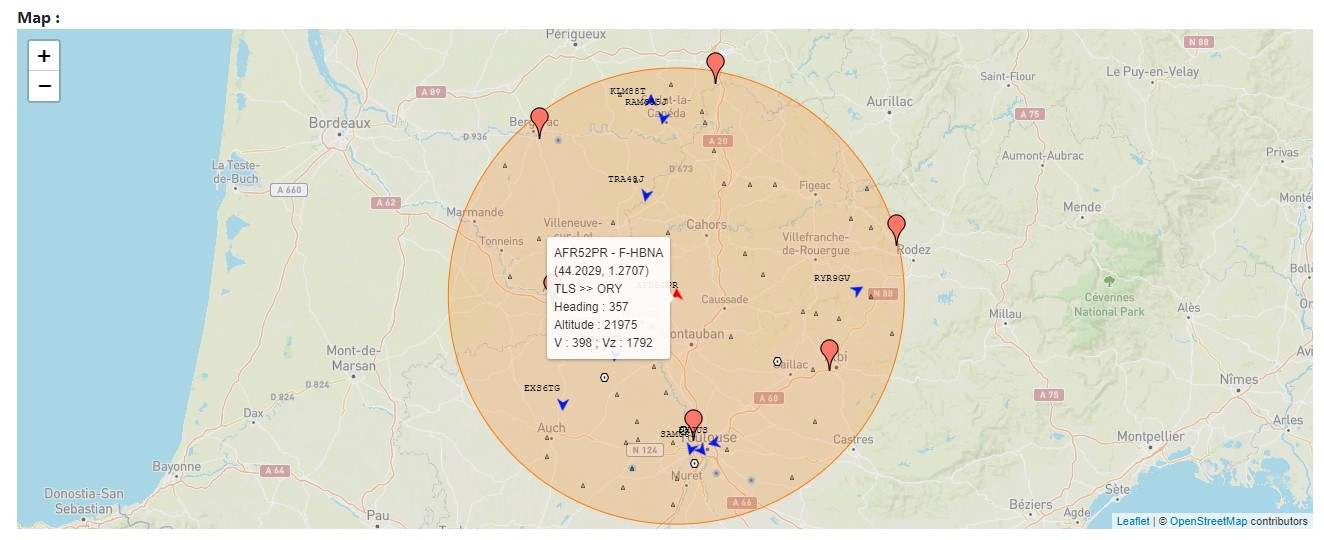
\includegraphics[width=.9\linewidth]{select_flight.jpg}
    \caption{Map after flight selection}
    \label{fig:select_flight}
\end{figure}


\subsection{Queries}
Once a flight is selected, you can ask queries to the flight assistant using the push-to-talk button, set to the '1' key of the character keys on your keyboard ('\&' key on an AZERTY keyboard). Queries can be asked either in natural language with plain sentences, or with sequence of specific words.

\begin{itemize}
    \item Push the push-to-talk button ('1' key) and maintain it.
    \item Ask your question. A transcript is also displayed in real-time.
    \item Release the push-to-talk button to send your query.
\end{itemize}

An exhaustive list of implemented queries with a list of possible questions are available at the \hyperref[sec:available-queries]{``Available queries''} section of this document
and indications on queries are provided in the following section.


% ------------------------------------------------------------------------------
\section{Queries}
\subsection{Static and dynamic queries}

\paragraph{Static queries}
For a selected flight, some data will not change.
By asking for your departure or arrival airport, the answer will remain the same for the duration of the flight.
In the same way, asking for information about an airport will return you the same answer.

\paragraph{Dynamic queries}
For this type of query, depending on your position, the evolution of the air traffic
and the weather, you will receive different answers during the flight.

\vspace{1em}

For these two types of queries, you only need to press the push-to-talk button, ask orally your request and
the flight assistant will answer you on the interface and orally.

\subsection{Checklists}

\textit{
Checklists queries have been partially implemented. These queries are only for test purposes.
}

\begin{itemize}
    \item Request one of the available checklists orally using the push-to-talk button. 
    \item A pop-up (Figure \ref{fig:checklist}) must appear, and an item is announced.
    \item \textbf{Without using again the push-to-talk button}, say the corresponding answer.
    \item If it is correct, the answer will be colored in green and the next item will be asked.
\end{itemize}



\begin{figure}[h!]
    \centering
    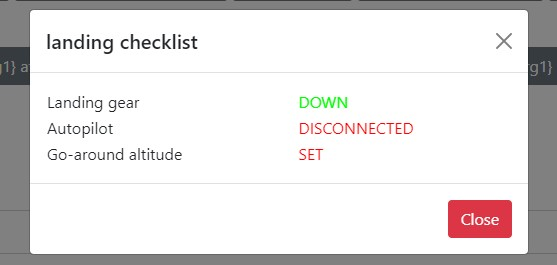
\includegraphics[width=.5\linewidth]{checklist.jpg}
    \caption{Checklist pop-up}
    \label{fig:checklist}
\end{figure}
% ------------------------------------------------------------------------------

\newpage
\begin{landscape}
\thispagestyle{empty}
\section*{Overview of the user interface}
\addcontentsline{toc}{section}{Overview of the user interface}

\begin{figure}[h!]
    \centering
    \resizebox{\linewidth}{!}{
        

\tikzset{every picture/.style={line width=0.75pt}} %set default line width to 0.75pt        

\begin{tikzpicture}[x=0.75pt,y=0.75pt,yscale=-1,xscale=1]
%uncomment if require: \path (0,522); %set diagram left start at 0, and has height of 522

%Image [id:dp26286327047717317] 
\draw (471,264) node  {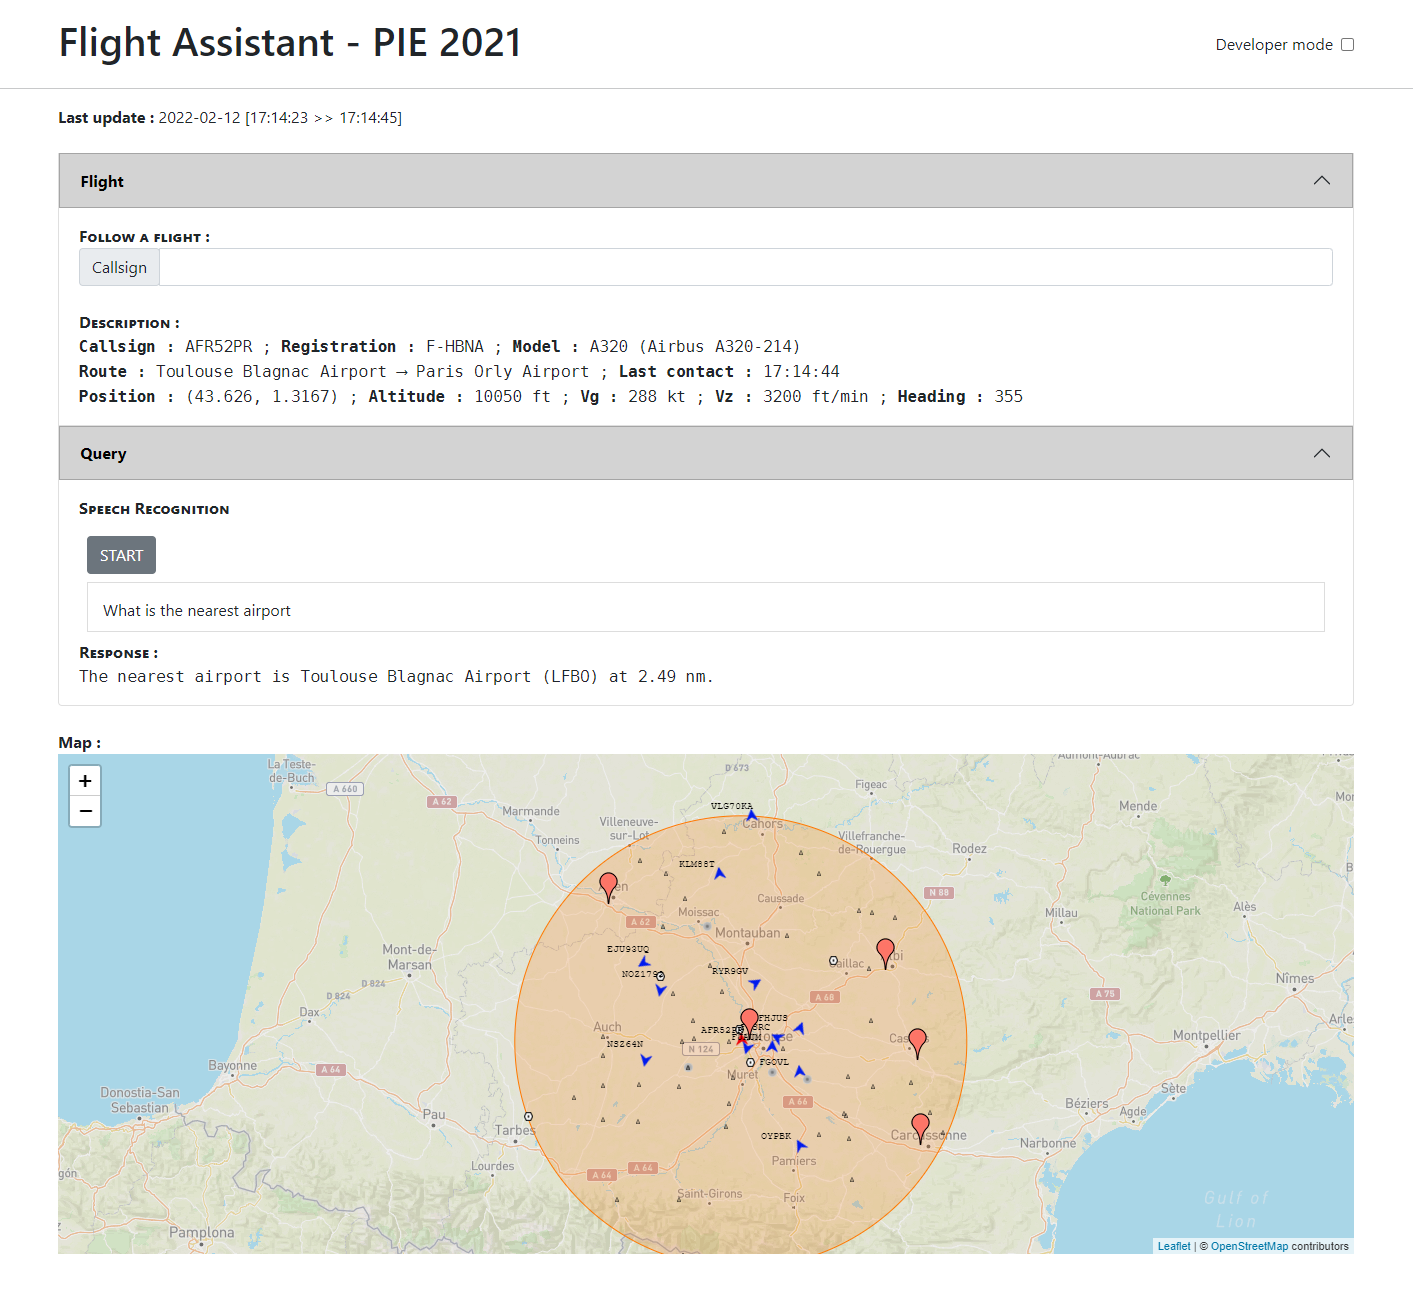
\includegraphics[width=376.5pt,height=376.5pt]{app.png}};
%Shape: Brace [id:dp6057064070284204] 
\draw   (730,178.5) .. controls (734.67,178.5) and (737,176.17) .. (737,171.5) -- (737,167.25) .. controls (737,160.58) and (739.33,157.25) .. (744,157.25) .. controls (739.33,157.25) and (737,153.92) .. (737,147.25)(737,150.25) -- (737,143) .. controls (737,138.33) and (734.67,136) .. (730,136) ;
%Straight Lines [id:da8707683011090381] 
\draw    (545,273) -- (729,273) ;
%Straight Lines [id:da25875277691433896] 
\draw    (198,227) -- (235,227) ;
%Straight Lines [id:da4807675461330312] 
\draw    (329,248) -- (726,248) ;
%Shape: Brace [id:dp3415007180555045] 
\draw   (214,302.5) .. controls (209.33,302.5) and (207,304.83) .. (207,309.5) -- (207,388.5) .. controls (207,395.17) and (204.67,398.5) .. (200,398.5) .. controls (204.67,398.5) and (207,401.83) .. (207,408.5)(207,405.5) -- (207,487.5) .. controls (207,492.17) and (209.33,494.5) .. (214,494.5) ;
%Straight Lines [id:da8544557884645487] 
\draw    (502,344) -- (741,344) ;
%Straight Lines [id:da49698209618690425] 
\draw    (521,369) -- (742,369) ;
%Straight Lines [id:da0380502625726169] 
\draw    (466,384) -- (826,384) ;
%Straight Lines [id:da8552163851908283] 
\draw    (508,433) -- (749,433) ;

% Text Node
\draw (757,150) node [anchor=north west][inner sep=0.75pt]   [align=left] {Flight information};
% Text Node
\draw (734,264) node [anchor=north west][inner sep=0.75pt]   [align=left] {Text query answer};
% Text Node
\draw (732,237) node [anchor=north west][inner sep=0.75pt]   [align=left] {Speech transcript};
% Text Node
\draw (7,207) node [anchor=north west][inner sep=0.75pt]   [align=left] {Speech Recognition trigger \\(or '1' key for push-to-talk)};
% Text Node
\draw (90,384) node [anchor=north west][inner sep=0.75pt]   [align=left] {Map with data\\in real-time};
% Text Node
\draw (749,336) node [anchor=north west][inner sep=0.75pt]   [align=left] {Traffic (blue arrow)};
% Text Node
\draw (748,362) node [anchor=north west][inner sep=0.75pt]   [align=left] {Airport };
% Text Node
\draw (834,377) node [anchor=north west][inner sep=0.75pt]   [align=left] {Selected traffic (red arrow)};
% Text Node
\draw (759,425) node [anchor=north west][inner sep=0.75pt]   [align=left] {Waypoints and navaids};


\end{tikzpicture}

    }
    \caption{User interface}
    \label{fig:user_interface}
\end{figure}
\end{landscape}







% ------------------------------------------------------------------------------
\newpage
\begin{landscape}
\thispagestyle{empty}
\section*{Available queries}
\label{sec:available-queries}
\addcontentsline{toc}{section}{Available queries}

Words between brackets can be changed. 
Available parameters (flight, weather, frequencies) are described in the next page.

\renewcommand{\arraystretch}{1.5}

\begin{table}[!h]

        \centering
        \footnotesize
\begin{tabular}{|p{0.2\paperwidth}|p{0.5\paperwidth}|p{0.4\paperwidth}|}
\hline
\rowcolor{gray} \textbf{Intent} & \textbf{Description} & \textbf{Examples} \\
\hline 

\rowcolor{lightgray} \multicolumn{3}{|l|}{Static queries (that will not change during the flight)} \\ \hline 
Departure / Arrival airport  & Returns the name and the ICAO of the departure / arrival airport & ``What is the arrival airport ?''  \\ 
\hline 
Runways at an airport  & Returns the list of runways at the an airport & ``What are the runways at [Toulouse Blagnac]* ?''  \\ 
\hline
Frequency at an airport  & Returns the frequency value of a frequency channel at an airport & ``[TWR] frequency at [Toulouse Blagnac]*''  \\ 
\hline

\rowcolor{lightgray} \multicolumn{3}{|l|}{Dynamic queries (that may change during the flight)} \\ \hline
Current flight parameters    & Returns a current flight parameter (speed, altitude, Vz, heading...)          &         ``What is my [altitude] ?''  \\
\hline
Nearest airport       & Returns the nearest airport from the current position &         ``What is the nearest airport ?''  \\ 
\hline
Nearest trafic       & Returns the nearest trafic from the current position &         ``Where is the nearest trafic ?''  \\ 
\hline
Nearest runways       & Returns the list of runways at the nearest airport &         ``What are the nearest runways ?''  \\ 
\hline
Length of the nearest runway       & Returns the length of the longest nearest runway &         ``What is the length of the nearest runway ?''  \\ 
\hline
Estimated time of arrival       & Returns the ETA &         ``Estimated time of arrival''  \\ 
\hline

\rowcolor{lightgray} \multicolumn{3}{|l|}{Weather queries} \\ \hline
Weather at airport       & Returns a global status of the weather or a specific parameter at an airport &         ``What is the weather at [Toulouse Blagnac]* ? \newline ``What is the [visibility] at [Toulouse Blagnac]* ?''  \\ 
\hline
Weather at location       & Returns a global status of the weather or a specific parameter at a location &         ``Give me the weather at [Toulouse] ?'' \newline ``[Temperature] at [Paris]''  \\ 
\hline
% Weather at waypoint       & Returns a global status of the weather or a specific parameter on the ground at a waypoint &         ``Weather at [OSKAM] ?'' \newline ``What is the [wind] at waypoint [OSKAM]''  \\ 
% \hline

\rowcolor{lightgray} \multicolumn{3}{|l|}{Checklists} \\ \hline
Approach checklist & Returns the approach checklist & ``Give me the approach checklist''  \\ 
\hline 
Landing checklist  & Returns the landing checklist & ``Landing checklist''  \\ 
\hline 
\end{tabular}

\end{table}

\noindent\rule{8cm}{0.4pt} \\
{\footnotesize * The airport can also be [arrival] or [departure]. \textbf{Current available airport names are French and English airports in this version.}}


% ------------------------------------------------------------------------------

\newpage
\thispagestyle{empty}

\subsection*{Available frequencies} 
(Depending on the airport) TWR (Tower), APP (Approach), GND (Ground), INFO, AFIS, ATIS

\subsection*{Available flight parameters} 
Heading, Speed, Altitude, Vertical speed, Latitude, Longitude, Callsign, Registration

\subsection*{Available weather parameters}
Temperature, Pressure, Wind, Gust, Clouds, Visibility, Rain, METAR


\end{landscape}




\end{document}